% IT4868E Web Mining — Capstone Final Report (draft, Group 20). ICLR 2027 template.
% Build:  make report   (runs report/make_tables.py, then tectonic; tables/ and numbers come from results/)
\documentclass{article}
\usepackage{iclr2027_conference}
\iclrfinalcopy
% Shared preamble for all Group 20 reports (ICLR 2027 template, XeLaTeX via tectonic).
% Usage:  \documentclass{article} \usepackage{iclr2027_conference} \iclrfinalcopy % Shared preamble for all Group 20 reports (ICLR 2027 template, XeLaTeX via tectonic).
% Usage:  \documentclass{article} \usepackage{iclr2027_conference} \iclrfinalcopy % Shared preamble for all Group 20 reports (ICLR 2027 template, XeLaTeX via tectonic).
% Usage:  \documentclass{article} \usepackage{iclr2027_conference} \iclrfinalcopy \input{common}
\usepackage{fontspec}
\setmainfont{texgyretermes}[Extension=.otf, UprightFont=*-regular, BoldFont=*-bold,
  ItalicFont=*-italic, BoldItalicFont=*-bolditalic]          % Times clone with Vietnamese glyphs
\usepackage{amsmath,amssymb}
\usepackage{unicode-math}
\setmathfont{texgyretermes-math.otf}
\usepackage{booktabs,tabularx,array}
\usepackage{graphicx}
\usepackage{subcaption}
\usepackage{tikz}
\usetikzlibrary{positioning,arrows.meta}
\usepackage{enumitem}
\usepackage{caption}
\usepackage{xcolor}
\definecolor{linkblue}{HTML}{1F4E9A}
\usepackage[colorlinks=true,linkcolor=linkblue,citecolor=linkblue,urlcolor=linkblue]{hyperref}
\usepackage{url}
\captionsetup{font=small,skip=3pt}
\setlist{nosep,leftmargin=1.2em}
\newcolumntype{L}[1]{>{\raggedright\arraybackslash}p{#1}}
\newcolumntype{Y}{>{\raggedright\arraybackslash}X}
\graphicspath{{../figures/}}
\raggedbottom

% ---- project macros -----------------------------------------------------------------------------
\newcommand{\repo}{\url{https://github.com/phunggiahuy159/vn-comparative-opinion-ranking}}
\newcommand{\todo}[1]{\textbf{[TODO: #1]}}
\newcommand{\groupauthors}{%
  Phùng Gia Huy \\ \textnormal{20235506} \And
  Vũ Hải An \\ \textnormal{20235468} \And
  Chu Xuân Minh \\ \textnormal{20235527} \And
  Nguyễn Bình Anh \\ \textnormal{20235470} \AND
  \textnormal{Hanoi University of Science and Technology} \\
  \textnormal{\texttt{\href{https://github.com/phunggiahuy159/vn-comparative-opinion-ranking}{github.com/phunggiahuy159/vn-comparative-opinion-ranking}}}}
% pipeline diagram, used by both reports
\newcommand{\pipeline}{%
\begin{tikzpicture}[node distance=0.22cm, every node/.style={font=\scriptsize},
  box/.style={draw, align=center, minimum height=0.8cm, text width=1.6cm, inner sep=2pt},
  arr/.style={-{Stealth[length=3.5pt]}, semithick}]
\node[box] (a) {Crawl reviews\\+ articles};
\node[box, right=of a] (b) {ABSA\\(PhoBERT)};
\node[box, right=of b] (c) {Comparative\\quintuples};
\node[box, right=of c] (d) {Entity\\linking};
\node[box, right=of d, very thick] (e) {\textbf{EDR ranking}\\+ intervals};
\node[box, right=of e] (f) {Benchmark\\correlation};
\foreach \x/\y in {a/b,b/c,c/d,d/e,e/f} \draw[arr] (\x) -- (\y);
\end{tikzpicture}}
\setlength{\bibsep}{1.5pt plus 0.5pt}                        % compact reference list

\usepackage{fontspec}
\setmainfont{texgyretermes}[Extension=.otf, UprightFont=*-regular, BoldFont=*-bold,
  ItalicFont=*-italic, BoldItalicFont=*-bolditalic]          % Times clone with Vietnamese glyphs
\usepackage{amsmath,amssymb}
\usepackage{unicode-math}
\setmathfont{texgyretermes-math.otf}
\usepackage{booktabs,tabularx,array}
\usepackage{graphicx}
\usepackage{subcaption}
\usepackage{tikz}
\usetikzlibrary{positioning,arrows.meta}
\usepackage{enumitem}
\usepackage{caption}
\usepackage{xcolor}
\definecolor{linkblue}{HTML}{1F4E9A}
\usepackage[colorlinks=true,linkcolor=linkblue,citecolor=linkblue,urlcolor=linkblue]{hyperref}
\usepackage{url}
\captionsetup{font=small,skip=3pt}
\setlist{nosep,leftmargin=1.2em}
\newcolumntype{L}[1]{>{\raggedright\arraybackslash}p{#1}}
\newcolumntype{Y}{>{\raggedright\arraybackslash}X}
\graphicspath{{../figures/}}
\raggedbottom

% ---- project macros -----------------------------------------------------------------------------
\newcommand{\repo}{\url{https://github.com/phunggiahuy159/vn-comparative-opinion-ranking}}
\newcommand{\todo}[1]{\textbf{[TODO: #1]}}
\newcommand{\groupauthors}{%
  Phùng Gia Huy \\ \textnormal{20235506} \And
  Vũ Hải An \\ \textnormal{20235468} \And
  Chu Xuân Minh \\ \textnormal{20235527} \And
  Nguyễn Bình Anh \\ \textnormal{20235470} \AND
  \textnormal{Hanoi University of Science and Technology} \\
  \textnormal{\texttt{\href{https://github.com/phunggiahuy159/vn-comparative-opinion-ranking}{github.com/phunggiahuy159/vn-comparative-opinion-ranking}}}}
% pipeline diagram, used by both reports
\newcommand{\pipeline}{%
\begin{tikzpicture}[node distance=0.22cm, every node/.style={font=\scriptsize},
  box/.style={draw, align=center, minimum height=0.8cm, text width=1.6cm, inner sep=2pt},
  arr/.style={-{Stealth[length=3.5pt]}, semithick}]
\node[box] (a) {Crawl reviews\\+ articles};
\node[box, right=of a] (b) {ABSA\\(PhoBERT)};
\node[box, right=of b] (c) {Comparative\\quintuples};
\node[box, right=of c] (d) {Entity\\linking};
\node[box, right=of d, very thick] (e) {\textbf{EDR ranking}\\+ intervals};
\node[box, right=of e] (f) {Benchmark\\correlation};
\foreach \x/\y in {a/b,b/c,c/d,d/e,e/f} \draw[arr] (\x) -- (\y);
\end{tikzpicture}}
\setlength{\bibsep}{1.5pt plus 0.5pt}                        % compact reference list

\usepackage{fontspec}
\setmainfont{texgyretermes}[Extension=.otf, UprightFont=*-regular, BoldFont=*-bold,
  ItalicFont=*-italic, BoldItalicFont=*-bolditalic]          % Times clone with Vietnamese glyphs
\usepackage{amsmath,amssymb}
\usepackage{unicode-math}
\setmathfont{texgyretermes-math.otf}
\usepackage{booktabs,tabularx,array}
\usepackage{graphicx}
\usepackage{subcaption}
\usepackage{tikz}
\usetikzlibrary{positioning,arrows.meta}
\usepackage{enumitem}
\usepackage{caption}
\usepackage{xcolor}
\definecolor{linkblue}{HTML}{1F4E9A}
\usepackage[colorlinks=true,linkcolor=linkblue,citecolor=linkblue,urlcolor=linkblue]{hyperref}
\usepackage{url}
\captionsetup{font=small,skip=3pt}
\setlist{nosep,leftmargin=1.2em}
\newcolumntype{L}[1]{>{\raggedright\arraybackslash}p{#1}}
\newcolumntype{Y}{>{\raggedright\arraybackslash}X}
\graphicspath{{../figures/}}
\raggedbottom

% ---- project macros -----------------------------------------------------------------------------
\newcommand{\repo}{\url{https://github.com/phunggiahuy159/vn-comparative-opinion-ranking}}
\newcommand{\todo}[1]{\textbf{[TODO: #1]}}
\newcommand{\groupauthors}{%
  Phùng Gia Huy \\ \textnormal{20235506} \And
  Vũ Hải An \\ \textnormal{20235468} \And
  Chu Xuân Minh \\ \textnormal{20235527} \And
  Nguyễn Bình Anh \\ \textnormal{20235470} \AND
  \textnormal{Hanoi University of Science and Technology} \\
  \textnormal{\texttt{\href{https://github.com/phunggiahuy159/vn-comparative-opinion-ranking}{github.com/phunggiahuy159/vn-comparative-opinion-ranking}}}}
% pipeline diagram, used by both reports
\newcommand{\pipeline}{%
\begin{tikzpicture}[node distance=0.22cm, every node/.style={font=\scriptsize},
  box/.style={draw, align=center, minimum height=0.8cm, text width=1.6cm, inner sep=2pt},
  arr/.style={-{Stealth[length=3.5pt]}, semithick}]
\node[box] (a) {Crawl reviews\\+ articles};
\node[box, right=of a] (b) {ABSA\\(PhoBERT)};
\node[box, right=of b] (c) {Comparative\\quintuples};
\node[box, right=of c] (d) {Entity\\linking};
\node[box, right=of d, very thick] (e) {\textbf{EDR ranking}\\+ intervals};
\node[box, right=of e] (f) {Benchmark\\correlation};
\foreach \x/\y in {a/b,b/c,c/d,d/e,e/f} \draw[arr] (\x) -- (\y);
\end{tikzpicture}}
\setlength{\bibsep}{1.5pt plus 0.5pt}                        % compact reference list

% generated by report/make_tables.py from results/ — do not edit
\newcommand{\NReviews}{1{,}894}
\newcommand{\NReviewsTGDD}{1{,}414}
\newcommand{\NReviewsCPS}{480}
\newcommand{\NProducts}{102}
\newcommand{\NLinkedComps}{23}
\newcommand{\MarginLow}{0.17}
\newcommand{\MarginHigh}{0.04}
\newcommand{\pRankGzero}{0.84}
\newcommand{\pRankGhigh}{0.66}
\newcommand{\ECE}{0.08}
\newcommand{\RealPriceBattery}{$-$0.10}
\newcommand{\RealPriceCamera}{$-$0.30}
\newcommand{\RealSentScreen}{0.66}


\title{Expectation--Disconfirmation Ranking:\\Mining Vietnamese Reviews to Rank\\Smartphones by Aspect}
\author{\groupauthors}

\begin{document}
\maketitle
\lhead{IT4868E Web Mining --- Group 20 --- Final Report}

\begin{abstract}
We study how to turn Vietnamese smartphone reviews into per-aspect product rankings (battery, camera, performance, screen)
that agree with objective benchmarks. Our pipeline extracts aspect-level sentiment with a multi-task PhoBERT model (0.815
aspect\#polarity micro-F1 on UIT-ViSFD, against 0.710 for TF-IDF), extracts comparative opinions, and links product mentions to a catalogue.
The prior approach ranks products by PageRank over a comparative-sentence graph (pRank). We show that it confounds popularity and
\emph{price-relative} sentiment (``ngon trong tầm giá'') with quality. We propose \textbf{Expectation--Disconfirmation Ranking (EDR)},
a joint model grounded in consumer-satisfaction theory. A latent quality explains both head-to-head comparisons (Bradley--Terry)
and sentiment, where sentiment reflects quality relative to the expectation set by price and brand. The degree of price-relativity
$\gamma$ is chosen by how well the model predicts held-out comparisons, and a Laplace posterior yields calibrated pairwise probabilities and rank intervals.
In controlled simulations EDR ties with pRank when reviewers judge absolutely and is the best ranker when sentiment is price-relative
(Spearman 0.82 vs.\ 0.66 for pRank). A break-even analysis shows that EDR stays clearly above ranking by price up to a 30\% extraction
error, while a Bradley--Terry + sentiment combination falls to the price baseline at about 10\%. On real data we report two behavioural findings: negative aspect mentions cost 1.5--2.7$\times$ more stars
than positive ones add (loss aversion), and buyers compare against their previous phone or a brand rather than against competitors.
\todo{one sentence on real benchmark / spec-proxy results}
\end{abstract}

%==================================================================================================
\section{Introduction}
Buyers read reviews to answer questions such as ``which phone has the best battery?''. Reviews contain the answer only implicitly.
Opinions target \emph{aspects} (\emph{``pin trâu nhưng camera chụp đêm kém''}), some are \emph{comparative}
(\emph{``pin trâu hơn con A50''}), and many are \emph{relative to expectations} (\emph{``ngon trong tầm giá''}: good \emph{for the price}).
A ranking that averages sentiment therefore answers ``which phone pleased its buyers most for what they paid?'', not ``which phone is best?''.

\paragraph{Contributions.}
(1)~A Vietnamese pipeline for aspect sentiment, comparative quintuples and product-mention linking, including implicit subjects.
(2)~An analysis of when graph rankers on the comparison graph reflect quality: PageRank and HITS mostly measure popularity, and pRank
\citep{zhang2010} tracks sentiment and degrades under price-relative sentiment.
(3)~EDR, which extends ranking on the same comparison graph: a theory-grounded joint model with interpretable parameters (hedonic price curve, price-relativity $\gamma$), where held-out comparisons select
the price-relativity, and with calibrated uncertainty.
(4)~A break-even analysis that links extraction accuracy (an NLP metric) to ranking quality (the end goal).
(5)~Behavioural findings on Vietnamese buyers.

%==================================================================================================
\section{Related work}
\paragraph{Aspect-based sentiment analysis} for Vietnamese is benchmarked by UIT-ViSFD \citep{visfd} (smartphone feedback, 10 aspects).
Pre-trained encoders such as PhoBERT \citep{phobert} are the standard backbone.
\paragraph{Comparative opinion mining} extracts relations $\langle$entity$_1$, entity$_2$, aspect, predicate, type$\rangle$ \citep{jindal2006}.
For Vietnamese, the VLSP~2023 ComOM shared task \citep{vcom} defines quintuples with 8 comparison labels.
\paragraph{Ranking from opinions.} \citet{zhang2010} build a per-feature graph from comparative sentences, weight nodes by the ratio of positive to negative
subjective sentences, and rank with pRank, a PageRank variant \citep{pagerank}; HITS \citep{hits} is the other classic link-analysis ranker. Paired-comparison models \citep{bt1952} rank from noisy pairwise outcomes, and \citet{tkachenko2014} model comparison direction and
entity ranking jointly in a generative model.
\paragraph{Expectations.} Expectation--disconfirmation theory \citep{oliver1980} models satisfaction as performance relative to expectation.
Prospect theory \citep{kt1979} adds loss aversion. \citet{lihitt2010} show empirically that review ratings mix quality with value for money
(price effects). We use these ideas to correct opinion-based product rankings, with comparisons used to estimate how price-relative the sentiment is.

%==================================================================================================
\section{Data}
\begin{itemize}
\item \textbf{UIT-ViSFD} \citep{visfd}: 11{,}122 annotated comments (7{,}786 / 1{,}112 / 2{,}224), 10 aspects + OTHERS, 3 polarities. Used to train and evaluate ABSA.
\item \textbf{Buyer reviews}, crawled from thegioididong.com (the source of ViSFD): \todo{final counts} reviews of \todo{N} models (2023--26),
plus listed prices and spec sheets. robots.txt was respected (5\,s delay), and no reviewer identities were stored.
\item \textbf{Expert articles}, from VnExpress (allowed by its robots.txt): phone reviews and comparisons. \todo{counts}
\item \textbf{Ground truth}: spec-sheet proxies (battery mAh, peak brightness) for all smartphones, and lab benchmarks
(GSMArena, DXOMARK, AnTuTu) for a subset. \todo{counts}
\end{itemize}

%==================================================================================================
\section{Method}
\subsection{Pipeline}
\begin{center}
\pipeline
\end{center}
\paragraph{ABSA.} PhoBERT-base-v2 with a shared encoder ([CLS] + mean pooling) and one 4-way head per aspect (none / positive / negative / neutral),
trained with a class-weighted loss. Word segmentation uses pyvi.
\paragraph{Comparative extraction.} The rule-based extractor uses comparative-sentence patterns \citep{jindal2006} adapted to Vietnamese
(\emph{hơn, không bằng, thua, ngang, nhất}), with predicate polarity that can reverse the direction (\emph{``nóng hơn''} $\Rightarrow$ worse).
An LLM extractor (Qwen2.5-7B-Instruct, few-shot, JSON output, VCOM labels) produces silver labels for higher recall.
\paragraph{Entity linking.} Each mention is mapped to a catalogue product, a brand set (\emph{``ss''}, \emph{``hơn samsung''}), or an external phone outside the catalogue.
The implicit subject is the reviewed product, or the article's title product.

\subsection{Expectation--Disconfirmation Ranking (EDR)}
Let $\theta_{p,a}$ be the latent quality of product $p$ on aspect $a$, i.e.\ what a benchmark would measure.
\begin{align}
\hat e_{p,a} &= \mathbf{x}_p^{\top}\mathbf{c}_a && \text{(hedonic expectation)}\\
\theta_{p,a} &\sim \mathcal N(\mu_p + \hat e_{p,a},\,\tau^2),\quad \mu_p\sim\mathcal N(0,\sigma_\mu^2) && \text{(empirical-Bayes prior)}\\
P(+\mid p,a) &= \sigma\!\big(\alpha_a(\theta_{p,a}-\gamma_a\,\hat e_{p,a}) + b_a\big) && \text{(disconfirmation)}\\
P(S_w\succ S_l) &= (1-\varepsilon_s)\,\sigma(\bar\theta_{S_w}-\bar\theta_{S_l}) + \varepsilon_s\,\sigma(\bar\theta_{S_l}-\bar\theta_{S_w}) && \text{(noisy Bradley--Terry)}
\end{align}
Here $\mathbf{x}_p$ holds the z-scored log price and brand indicators, $S$ is a product or a brand set ($\bar\theta$ is the set mean), and $\varepsilon_s$ is the
direction-error rate of source $s$, measured on gold annotations. Sentiment counts enter through a binomial likelihood.
\paragraph{Interpretation.} $\gamma_a\in[0,1]$ is a \emph{price-relativity index}: $\gamma=0$ means absolute judgements, and $\gamma=1$ means ``good for the price''.
\paragraph{Selecting $\gamma$.} Learned jointly, $\gamma$ is weakly identified (Section~\ref{sec:synthetic}).
Head-to-head comparisons are not price-relative, so we choose $\gamma$ from a grid by $K$-fold held-out comparison log-likelihood.
\paragraph{Inference.} We fit by MAP (L-BFGS). A Laplace approximation of the posterior over $\boldsymbol\theta$ gives $P(\theta_i>\theta_j)$ and credible rank intervals.

%==================================================================================================
\section{Experiments}
\subsection{ABSA (UIT-ViSFD test set)}
\begin{center}\small
\setlength{\tabcolsep}{5pt}% generated by report/make_tables.py from results/ — do not edit
\begin{tabular}{@{}lcccccc@{}}
\toprule
UIT-ViSFD test, micro-F1 & Detection & Aspect\#polarity & Battery & Camera & Perf. & Screen \\
\midrule
TF-IDF + multinomial NB & 0.709 & 0.600 & -- & -- & -- & -- \\
TF-IDF + linear SVM & 0.822 & 0.713 & -- & -- & -- & -- \\
TF-IDF + logistic regression & 0.829 & 0.710 & -- & -- & -- & -- \\
PhoBERT-base-v2, multi-task & \textbf{0.890} & \textbf{0.815} & 0.856 & 0.870 & 0.829 & 0.771 \\
\bottomrule
\end{tabular}
\end{center}
\todo{add PhoBERT-large / XLM-R rows, 3 seeds (Kaggle)}

\subsection{Controlled simulation}\label{sec:synthetic}
The simulated world has 40 phones in 6 brands. True quality follows a hedonic market, and sentiment is price-relative with strength $\gamma$.
Comparisons follow Bradley--Terry with Zipf-like popularity; 30\% of them name only a brand, and extraction flips their direction with rate $\varepsilon$.
\begin{table}[h]\centering\footnotesize\setlength{\tabcolsep}{5pt}
\caption{Spearman $\rho$ against true quality, mean over 20 seeds ($\varepsilon=0.1$, 300 comparisons per aspect). Columns: true price-relativity $\gamma$.}\label{tab:e1}
% generated by report/make_tables.py from results/ — do not edit
\begin{tabular}{@{}lccc@{}}
\toprule
Ranker & $\gamma{=}0$ & $\gamma{=}0.5$ & $\gamma{=}0.8$ \\
\midrule
Price only & 0.634 & 0.634 & 0.634 \\
Sentiment only & 0.838 & 0.777 & 0.661 \\
PageRank & 0.136 & 0.136 & 0.136 \\
HITS & 0.103 & 0.103 & 0.103 \\
pRank & 0.841 & 0.778 & 0.664 \\
Bradley--Terry (BT) & 0.521 & 0.521 & 0.521 \\
BT + sentiment & 0.746 & 0.725 & 0.677 \\
\textbf{EDR (ours)} & \textbf{0.855} & \textbf{0.833} & \textbf{0.818} \\
\midrule
\quad $-$ $\gamma$ fixed at 0 & 0.856 & 0.789 & 0.683 \\
\quad $-$ $\gamma$ learned jointly & 0.809 & 0.810 & 0.808 \\
\quad $-$ no hedonic prior & 0.829 & 0.811 & 0.808 \\
\quad selected $\gamma$ & 0.17 & 0.47 & 0.60 \\
\bottomrule
\end{tabular}
\end{table}

\begin{figure}[h]
\centering
\begin{subfigure}{0.49\textwidth}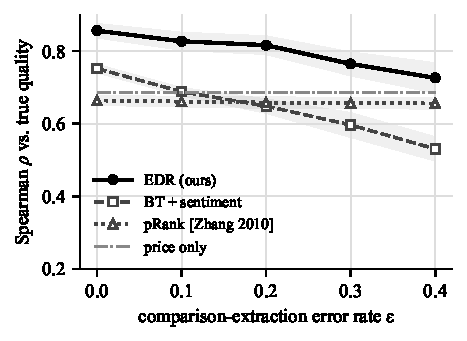
\includegraphics[width=\linewidth]{breakeven.pdf}\caption{Break-even ($\gamma=0.8$).}\end{subfigure}
\begin{subfigure}{0.49\textwidth}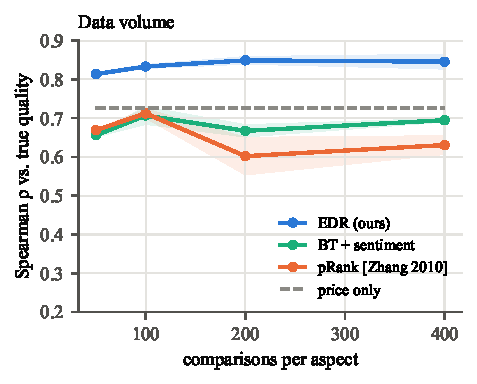
\includegraphics[width=\linewidth]{sparsity.pdf}\caption{Data volume ($\gamma=0.8$, $\varepsilon=0.1$).}\end{subfigure}
\begin{subfigure}{0.34\textwidth}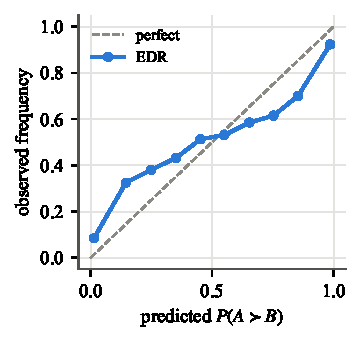
\includegraphics[width=\linewidth]{calibration.pdf}\caption{Calibration.}\end{subfigure}
\caption{Synthetic results (mean $\pm$ s.e.). EDR stays clearly above ranking by price up to $\varepsilon=0.3$ (margin \MarginLow{} at $\varepsilon=0$); at $0.4$ the margin (\MarginHigh{}) is within noise. Bradley--Terry + sentiment
falls below price at $\varepsilon\approx0.1$, and pRank tracks sentiment. EDR's pairwise probabilities are roughly calibrated (ECE \ECE) but somewhat overconfident at the extremes.}
\end{figure}

\subsection{Real data}
\paragraph{Corpus.} We crawl all 279 phone pages listed on thegioididong.com (1{,}414 usable reviews of 102 models) and add
480 reviews of 59 of these models from CellphoneS, for 1{,}894 reviews in total; 43 models have at least 10 reviews.
Spec sheets give ground-truth proxies for 66 (battery), 55 (screen) and 86 (camera) models.
The rules find 23 linked comparisons, none between two catalogue phones, so on buyer reviews alone EDR runs without head-to-head evidence
and $\gamma$ cannot be selected by held-out comparisons (we fall back to the joint estimate).

\begin{table}[h]\centering\small\setlength{\tabcolsep}{4pt}
\caption{Preliminary real-data results: Spearman $\rho$ (95\% bootstrap CI) between each ranking and the spec-sheet proxy,
smartphones with ${\ge}10$ reviews from both stores. Without head-to-head comparisons, PageRank, HITS and Bradley--Terry are undefined.}\label{tab:real}
% generated by report/make_tables.py from results/ — do not edit
\begin{tabular}{@{}llcccc@{}}
\toprule
Aspect & Proxy ($n$) & Price only & Sentiment & pRank & EDR \\
\midrule
Battery & mAh (23) & $-$0.10 {\scriptsize[$-$0.50, 0.35]} & 0.04 {\scriptsize[$-$0.36, 0.46]} & 0.06 {\scriptsize[$-$0.32, 0.45]} & 0.06 {\scriptsize[$-$0.31, 0.45]} \\
Screen & peak nits (21) & 0.63 {\scriptsize[0.18, 0.91]} & 0.66 {\scriptsize[0.40, 0.83]} & 0.66 {\scriptsize[0.40, 0.84]} & 0.55 {\scriptsize[0.11, 0.81]} \\
Camera & main MP, weak (35) & $-$0.30 {\scriptsize[$-$0.65, 0.09]} & 0.24 {\scriptsize[$-$0.04, 0.48]} & 0.23 {\scriptsize[$-$0.04, 0.47]} & 0.18 {\scriptsize[$-$0.15, 0.47]} \\
\bottomrule
\end{tabular}
\end{table}

\paragraph{Discussion.} Price fails where the simulation predicts: budget phones have the biggest batteries and the most megapixels,
so ranking by price is negatively correlated with both. Review-based rankings recover a clear signal only for the screen, and
EDR does not improve on sentiment ranking here: without comparisons it cannot tell price-relative from absolute praise. With about 20 phones per aspect and
mostly fewer than 10 aspect mentions per phone, the confidence intervals overlap and the rankers are not yet distinguishable.
\todo{rerun with expert-article comparisons (LLM extraction); chip $\to$ AnTuTu for performance}

\section{Findings about Vietnamese buyers}
\paragraph{Loss aversion.} Regressing star ratings on aspect polarity in ViSFD ($R^2=0.615$, $n=11{,}122$) shows that negative mentions cost
1.5--2.7$\times$ more stars than positive mentions add (e.g.\ PERFORMANCE $+0.40/-0.61$). DESIGN is the exception ($+0.31/-0.17$).
\paragraph{Reference points.} In buyer reviews, comparisons target the reviewer's \emph{previous} phone or a \emph{brand}, and almost never a competing current
model, so head-to-head evidence must come from expert text.
\paragraph{Two questions.} Buyer sentiment ranks \emph{value for money}, whereas benchmarks rank \emph{absolute quality}. EDR separates the two.

\section{Limitations and ethics}
Simulations show mechanisms, not real-world accuracy. Spec proxies (mAh, nits) are imperfect stand-ins for lab tests.
Review counts per phone are modest. All crawling followed robots.txt with rate limits; we skipped a site that disallows our crawler and stored no personal data.

\section{Conclusion}
\todo{after real results}

{\small
\bibliographystyle{iclr2027_conference}
\bibliography{refs}}
\end{document}
